\capitulo{6}{Trabajos relacionados}

\section{IP Cam Viewer Lite}

IP Camera Viewer Lite (figura \ref{fig:hitmob}) es una aplicación android que permite acceder y controlar remotamente su cámara IP, grabador de vídeo digital, grabador de red y/o cámara web. Es un proyecto realizado por \href{https://hit-mob.com}{\textit{hit-mob.com}} con la colaboración de \href{https://wordpress.com}{\textit{WordPress}}.

\begin{figure}[h!]
	\centering
	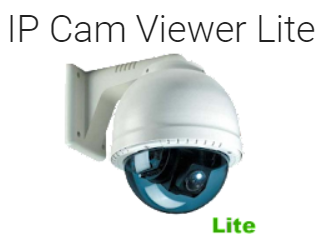
\includegraphics[width=0.35\linewidth]{img/ipCamViewerLite}
	\caption{Logo de la aplicación \textit{IP Cam Viewer Lite}.}
	\label{fig:hitmob}
\end{figure}

Esta aplicación es muy parecida a la que en este proyecto se ha desarrollado pero es muy compleja de utilizar, y requiere tener ciertos conocimientos sobre la red de internet y sus protocolos y conexiones.\\

Puedes encontrar dicha aplicación en el siguiente enlace: \href{https://play.google.com/store/apps/details?id=com.rcreations.ipcamviewer}{\textit{IP Cam Viewer Lite}}.



\section{tinyCam Monitor PRO}

tinyCam Monitor (figura \ref{fig:tinyCam}) es una aplicación desarrollada para el sistema Android diseñada con el fin de poder vigilar, controlar y grabar remotamente vídeo digital para cámaras de red o IP (ya sean privadas o públicas), DVRs y/o codificadores de vídeo.
Esta aplicación ha sido desarrollada por \href{https://tinysolutionsllc.com}{\textit{Tiny Solutions LLC}}.

\begin{figure}[h!]
	\centering
	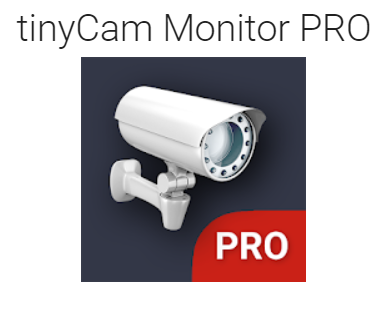
\includegraphics[width=0.35\linewidth]{img/tinyCam-Monitor-PRO}
	\caption{Logo de la aplicación \textit{tinyCam Monitor PRO}.}
	\label{fig:tinyCam}
\end{figure} 

tinyCam Monitor PRO tiene una interfaz de usuario mucho más simple y fácil de usar que IP Cam Viewer Lite pero es de pago.

Puedes encontrar dicha aplicación en el siguiente enlace: \href{https://play.google.com/store/apps/details?id=com.alexvas.dvr.pro&hl=es&gl=US}{\textit{tinyCam Monitor PRO}}.



\section{Ventajas y debilidades respecto a la competencia}


\begin{table}[h!]
\centering
\begin{tabular}{lccc}
\toprule
Características                 & AppFran     & IP Cam Viewer Lite & tinyCam Monitor PRO   \\
\midrule
Servidor en local               & \cellcolor{green!25} {$\checkmark$} & \cellcolor{red!25} {$\times$}  & \cellcolor{red!25} {$\times$}  \\
Interfaz de usuario             & \cellcolor{green!25} {$\checkmark$} & \cellcolor{red!25} {$\times$}  & \cellcolor{green!25} {$\checkmark$}  \\
Gratuito                        & \cellcolor{green!25} {$\checkmark$} & \cellcolor{green!25} {$\checkmark$}  & \cellcolor{red!25} {$\times$}  \\
Log                        & \cellcolor{green!25} {$\checkmark$} & \cellcolor{red!25} {$\times$}  & \cellcolor{red!25} {$\times$}  \\
Plataformas                     & Android    & Android     & Android     \\
\bottomrule
\end{tabular}
\caption{Comparativa de las características de los proyectos.}
\label{comparativa-proyectos}
\end{table}

Las principales fortalezas del proyecto son:

\begin{itemize}
\tightlist
\item
  \textbf{Servidor en local}: en este proyecto no se envían las imágenes a ningún servidor remoto, no sale de nuestro router la información. Esto es una ventaja ya que muchas empresas dedicadas a la monitorización de cámaras primero envían las imágenes a sus servidores que pueden estar en cualquier lugar del mundo (normalmente china) y desde ese servidor envían las imágenes a nuestra aplicación conectada a Internet, con la consiguiente pérdida de rendimiento.
\item
  \textbf{Interfaz de usuario}: la interfaz de usuario de la aplicación es muy intuitiva, sencilla y con una curva de aprendizaje rápida y accesible a todo el mundo, incluso sin conocimiento previo del tema.
\item
  \textbf{Aplicación gratuita}.
\end{itemize}

Las principales debilidades son:

\begin{itemize}
\tightlist
\item
  Tiene menos funcionalidades que la competencia
\item
  Menor calidad de imagen.
\end{itemize}





